\documentclass[10pt,letter]{article}
\usepackage{amsmath}
\usepackage{amssymb}
\usepackage{graphicx}
\usepackage{setspace}
\onehalfspacing
\usepackage{fullpage}
\newcommand{\R}{\mathbb{R}}	
\newcommand{\inner}{\langle\cdot,\cdot\rangle}
\newcommand{\inr}[2]{\langle #1, #2\rangle}
\newcommand\norm[1]{\left\lVert#1\right\rVert}

\graphicspath{ {images/} }

\begin{document}


\title{CS142 Homework Set \#4 Solutions}

\author{Timur Kuzhagaliyev}

%\date{24th October, 2017}
 
\maketitle 

\section*{Problem 1}

Concurrency is not transitive. Here is a counterexample. Suppose $A, B, C$ are
events on the timelines of processes $P, Q, R,$ respectively. $P$ sends a message to $R$ after event
$A$ and the message is received before event $C$. So there is a path from $A$ to $C$. Event $B$ is the
beginning local event on process $Q$; at this point $Q$ has not sent or received messages from
any agent. So, there is no path to or from event $B$. So $B$ is concurrent with $A$ and with $C$,
while $A$ and $C$ are clearly not concurrent.

\section*{Problem 2}

Solution to problem 2:

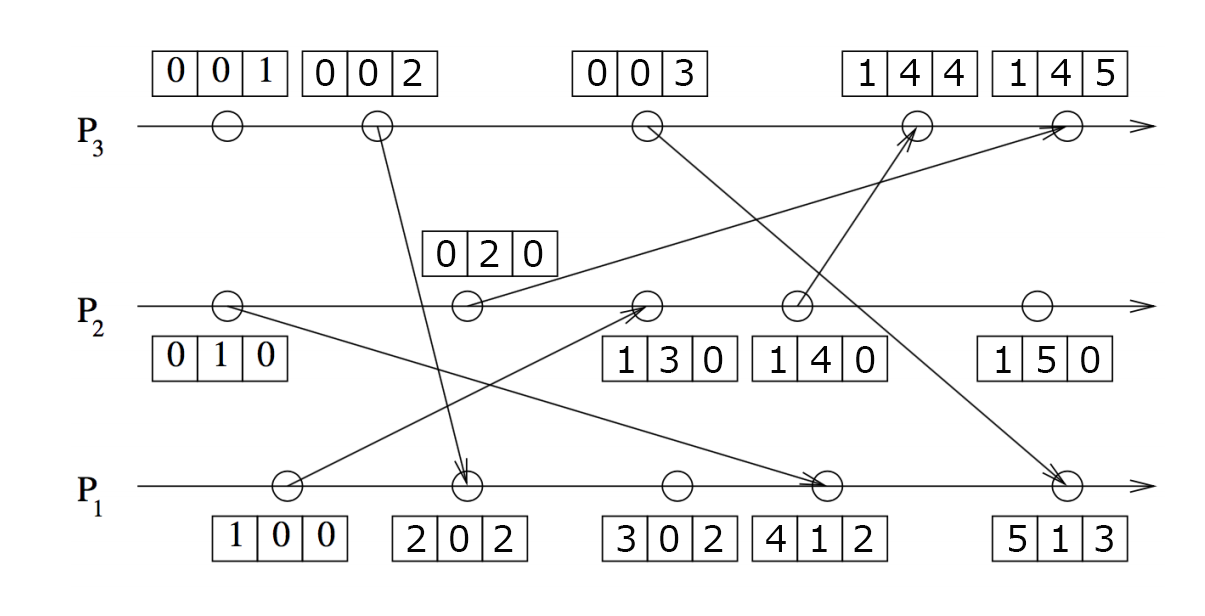
\includegraphics[width=\textwidth,height=\textheight,keepaspectratio]{hw4_problem2}

\section*{Problem 3}

\paragraph{a)} The algorithm is correct. We're told that the OS can observe the state of the entire distributed system at any point in time, including both agent and channel states. Note that the system terminates when all channels are empty and and all agents are idle, and we also know that $\textbf{stable}(terminated)$.

By definition of our algorithm, once the OS observes that $terminated$ holds (which can happen at most $T$ units of time after actual termination), it will set the value of $claim\_terminated$ to $true$. Clearly, the progress property holds as $terminated \leadsto claim\_terminated$.

Denote the point in time when the OS observes $terminated = true$ as $T_0$. By definition of the algorithm, $claim\_terminated$ is false up until $T_0$, so by definition of implication $claim\_terminated \Rightarrow terminated$ is $true$ up until $T_0$. At and after $T_0$, $terminated$ is $true$ (by definition of $T_0$) and OS sets $claim\_terminated$ to $true$ also. Since $terminated$ is stable, it will remain $true$, and by definition of our algorithm so will $claim\_terminated$. This means that at and after $T_0$ the predicate $claim\_terminated \Rightarrow terminated$ still evaluates to $true$. Since together time intervals before and after $T_0$ make up the whole time domain, $claim\_terminated \Rightarrow terminated$ always holds and hence is invariant. Therefore the safety property is satisfied.

By the two points above, the algorithm is correct.

 \paragraph{b)} This algorithm is wrong, and here is a simple counterexample. Suppose $D$ has two agents, $A$ and $B$, with two directed channels between them. Initially, both $A$ and $B$ are active and the channels are empty. Agent $B$ goes idle, and sends $(B, 0, 0)$ to the OS. Agent $A$ sends a message to $B$, which activates B again, and make it send another message to A. After receiving the message, A goes idle, and sends $(A, 1, 1)$ to the OS. At this point, the OS has received one message from each agent, and further

\[
\sum\limits_{r} r.count\_received = \sum\limits_{r} r.count\_sent = 1 + 0
\]

As a result, the OS sets $claim\_terminated$ to $true$, but agent $B$ is still active, and
$terminated$ is $false$. Therefore, the safety condition is violated.

 \paragraph{c)} \textbf{Proving invariant}: We know that $claim\_terminated$ is initially false and will remain false until OS observes all necessary properties. Denote the moment when OS sets $claim\_terminated$ to true as $T_0$. Clearly, before $T_0$ $claim\_terminated \Rightarrow terminated$ holds by definition of implication.

We know that $terminated$ is stable, so if we can show that at $\tau = T_0$ the conditions observed by the OS indeed show that the system has terminated, we can infer that the system will remain terminated. We can prove that by contradiction. We know that at time $\tau$ (with respect to each agent's individual logical clock) all agents were inactive. The only thing that could activate them afterwards was an incoming message. Assume there was indeed an agent that got activated after our observation. For this to be possible, someone must have sent a message to activate, and there are two ways this could happen:

\begin{itemize}
\item The message was sent before time $\tau$. If the message was sent before $\tau$, one of the agents would have incremented their sent message counter by one. Since the message would still be in flight at $\tau$, the total sum of all received messages would be 1 count below the total sum of all sent messages, which contradicts the observation of the OS.
\item The message was sent after time $\tau$. For this to be possible there must be at least one active agent after $\tau$, which is not the case as seen in our observation.
\end{itemize}

Hence, by contradiction, no agent can become active after $T_0$ and all channels must be empty. This implies that the system has terminated, and $claim\_terminated \Rightarrow terminated$ holds. Therefore $claim\_terminated \Rightarrow terminated$ is invariant. Note that we used the idea explained in part b), namely the $\sum\limits_{r} r.count\_received \leq \sum\limits_{r} r.count\_sent$ invariant.

\textbf{Showing progress}: We're given that the logical clock on each agent increments eventually, and each agent reports its state to OS after every interval $T$ with respect to its own clock. Let $T_{max}$ be the longest of intervals $T$ of all agents, in absolute time units. Since the agents report their progress periodically, once the system terminates, we know that OS will see the state of all agents after termination at most after $T_{max}$ absolute units of time after the actual termination occurred.

When $terminated$ holds, we know that all agents are idle and all channels are empty. It is clear that agents will report their states as idle, what satisfies one property of OS termination claim. Since there are no messages in channels, all sent messages must have been received, so total sum of sent messages is equal to total sum of received messages, what satisfies the second property of OS termination claim. Hence OS will set the $claim\_terminated$ to true. This shows that the algorithm satisfies the progress property $terminated \leadsto claim\_terminated$.

By the 2 points above, the algorithm is correct.

\end{document}